\section{Preliminaries}

\begin{itemize}
\item Discussion paper (Cross Validation Gone Wrong)
\end{itemize}

\section{Motivation}

Part of what makes machine learning exciting is the availability of flexible models which can better predict complex phenomena. 
However, the possibility of overfitting complicated our enthusiasm for complicated models. For example, we saw scenarios where cross validation will lead us to select a simple
intercept-only model instead of a complicated polynomial model when applying linear regression. 

This helps avoid ugly scenarios like in the figure below, where a polynomial fit probably won't generalize well.

\begin{center}
    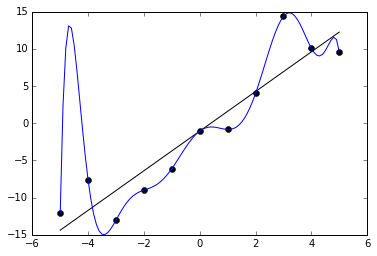
\includegraphics[width = .6\textwidth]{images/Overfitted_Data.png}
\end{center}


Regularization offers a\footnote{\emph{a}, not \emph{the}} middle path where we can smooth out these wild predictions without necessarily dropping as many predictors and without needing to compare the $2^p$ model specifications you might select as subsets among $p$ predictors. 

In these notes, we introduce 

\begin{itemize}
    \item Ridge (L2) regularization
    \item LASSO (L1) regularization
    \item Double LASSO variable selection
\end{itemize}

Lasso has no general, closed form solution and the ``current distribution theory of lasso esimation is challenging'' according to Bruce Hansen, so we restrict most of our analytical endeavors to ridge. 

\section{Main Points}

Ridge and lasso are two regularization methods that we can apply to linear regression. These are \emph{penalized} models, where we modify the loss function to increase the loss according to the magnitude of the slope parameters.

The penalty is a scalar-valued hyperparameter that we can tune with cross validation. Both ridge and lasso reduce the coefficients and they can be helpful in cases of collinearity or where you have more predictors than observations. 
Lasso is useful for model selection because it tends to select sparse solutions, meaning many parameters are set to be zero. Ridge does not do this, but it is more tailored for dealing with multicollinearity. 

Apply these methods using code like below.

\begin{lstlisting}
from sklearn.linear_model import Ridge, Lasso, LinearRegression

# Create collinear data
X = [[0,0], [1, 1], [2, 2]]
y = [100, 101, 102]

# Initialize models
m_ols = LinearRegression()
m_ridge = Ridge(alpha=10e-4) # alpha is the penalty (=0 for OLS)
m_lasso = Lasso(alpha=10e-8)

# Fit and inspect
for m in m_ols, m_ridge, m_lasso:
    m.fit(X, y)
    print()
    print(m.intercept_)
    print(m.coef_)
\end{lstlisting}


$$
\begin{array}{lccc}
\text{Model} & \text{Intercept} & \text{Coefficient 1} & \text{Coefficient 2} \\
\hline
\text{OLS} & 100.0 & 0.5 & 0.5 \\
\text{Ridge } (\alpha = 10^{-3}) & 100.00025 & 0.49988 & 0.49988 \\
\text{Lasso } (\alpha = 10^{-7}) & 100.00000015 & 0.99999985 & 0
\end{array}
$$

Note, the intercept is usually not penalized. To ensure the penalty applies equally to each predictor, it is typical to convert each predictor into standard units before fitting the regression. Dummy variables might be left untransformed and the target is usually not changed.


There are a few surprises as we delve deeper. For example, ridge regression will shrink coefficients for weak predictors more than strong predictors, but the shrinkage is not more severe for data with more irreducible noise. 

\section{Ridge Regression}

Consider a regression problem where we have an $n\times p$ design matrix $X$ and we want to find the coefficients $w$. 

Recall OLS finds

$$ w_{OLS} = \arg\min_w \Vert Y - Xw \Vert_2^2.$$

Ridge regression finds

$$ w_{ridge} = \arg\min_w \Vert Y - Xw \Vert_2^2 + \lambda \Vert w \Vert_2^2, $$

where $\lambda \in \mathbb{R}_+$ is the penalty or regularization strength. Note that if $\lambda = 0$, we return to OLS. As $\lambda \rightarrow \infty$, $w$ will approach the zero vector. $\lambda$ is a hyperparameter. 

If we have just one predictor, we can write the right hand side more simply as

$$ \sum_{i=1}^n (y - wx_{i})^2 + \lambda w^2. $$

The solution to this is analytically straightforward (we aren't interested in the derivation though). This even works for $p>n$. 


$$w_{ridge} = (X^TX + \lambda I)^{-1} X^TY.$$


We are minimizing the usual loss function but we are paying a price for an increase in $w$.
The cost is based on the L2 (Euclidean) norm. This means that the marginal cost of increasing $w$ is $2\lambda w$.
At $w=0$, the marginal penalty of increasing or decreasing $w$ by an infinitesimal amount is zero. 
Therefore, nonzero coefficnets tend to stay nonzero for moderate choices of $\lambda$. 

It's easier to see this with a hand-wavy proof by picture based on the equivalent constrained minimization problem. 
The modified loss function we are minimizing above is unconstrained, but the value of $\lambda$ corresponds to a different problem where we have a budget $\tau$ to ``spend'' on each coefficient. 

$$\min_{w} \Vert Y - Xw \Vert_2^2 \text{ subject to } \Vert w \Vert_2 ^2 \leq \tau. $$


\begin{center}
    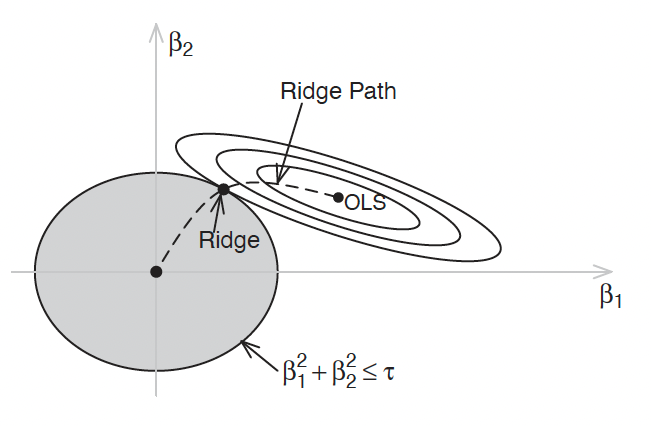
\includegraphics[width=.7\textwidth]{images/ridge_dual.png}
\end{center}


\subsection{Orthonormal Problems}

Ridge regression was first introduced with cases of ``nonorthogonality'' in mind. That is, where the Gram matrix $X^T X$ has non-zero elements off the diagonal. That is, where columns of $X$ are correlated.
Recall that for standardized columns $i$ and $j$, $x_j^T x_i = n\rho$, where $\rho$ is their (population) correlation coefficient.  Briefly, we'll consider the case where $X$ columns are uncorrelated so we have zeros off the diagonal. 


In general, $$w_{ridge} = (X^T X + \lambda I)^{-1} X^T Y.$$

Suppose that $X^T X = I$, then

$$w_{ridge} = (I + \lambda I)^{-1} X^T Y = ((1+\lambda)I)^{-1}X^T Y = \frac{1}{1+\lambda} (X^T X)^{-1} X^T Y= \frac{1}{1+\lambda} w_{ols}.$$

Ridge scales down each coefficient by a factor $\frac{1}{1+\lambda}$. This depends on the particular assumption $X^TX$. In the general orthogonal case, $X^TX$ is not necessarily $I$, but it will be a matrix with only diagonal terms. 

When columns of $X$ are orthogonal, $X^TX = \text{diag}(d_1, \ldots, d_p)$ where the $d_i$ on the diagonal happen to be the eigenvalues of the Gram matrix, giving:
$$w_{ridge}^{(i)} = \frac{d_i}{d_i + \lambda} w_{ols}^{(i)}.$$

When $d_i$ is large, notice that the shrinkage is not severe. When $d_i \ll \lambda$, then the coefficient is scaled down nearly to zero. 

\subsubsection{Standardizing Columns (orthogonal case)}

We just learned that if $d_i \gg \lambda$, then the coefficient doesn't change much.

Suppose a villain is in charge of your data preprocessing and doesn't want the coefficient for the first column to change. What would that villain do? He might scale that column by some value $s$. If he chooses $s$ to be large, 
he is increasing the variance in the first dimension. This corresponds to a high $d_1$ (eigenvalue). Therefore, $\frac{d_1}{d_1 + \lambda} \approx 1$ and $w_{ridge}^{(1)} \approx w_{ols}^{(1)}$


The solution is to do your own preprocessing and standardize your columns ($x\leftarrow \frac{x-\bar{x}}{s_x}$).


\subsection{Nonorthogonal}

When $X^TX$ has off-diagonal elements (correlations), we need the eigendecomposition to proceed analytically.

$$X^TX = V\Lambda V^T$$

Then:
$$w_{ridge} = V \text{diag}\left(\frac{\lambda_1}{\lambda_1 + \lambda}, \ldots, \frac{\lambda_p}{\lambda_p + \lambda}\right) V^T w_{ols}$$

This means:
\begin{enumerate}
    \item Transform $w_{ols}$ to the eigenvector basis: $V^T w_{ols}$
    \item Apply shrinkage in that basis: scale by $\frac{\lambda_i}{\lambda_i + \lambda}$  
    \item Transform back: multiply by $V$ ($V$ and $V^T$ are inverses)
\end{enumerate}

Shrinkage happens along \emph{eigenvector directions}, not coordinate directions. You don't have to understand eigendecompositions deeply to understand something interesting: the shrinkage is determined by properties of $X^TX$ alone.

The irreducible noise built into $Y$ that is not in $X$ will not change the shrinkage. 


These two scenarios will produce loss surfaces that are similar in that we should find parameters $w^T = (1, 3)$ in expectation. 

\begin{enumerate}
    \item $y_i = x_1 + 3x_2 + \epsilon$, $\epsilon \sim N(0,1)$
    \item $y_i = x_1 + 3x_2 + \epsilon$, $\epsilon \sim N(0,10000)$
\end{enumerate}

It would be reasonable to expect the loss surface for the second one to be flatter. Thus, you would reason that a fixed penalty $\lambda$ would shrink the coefficients more in the second case. This is not what happens though!.
Shrinkage depends on the curvature of the loss surface, and this only depends on $X$. 

$$\nabla L(w) = X^T(Xw - Y) = 2X^TXw - 2X^TY$$

$$\nabla^2 L(w) = 2X^TX$$

The values of $Y$ will change the level and slope along the loss surface, but not the curvature.

The Hessian (second derivative) describes the curvature, depending only on $X$. And it is the curvature that affects shrinkage. 


\section{LASSO}

LASSO (L1) penalization solves
\[
w_{\text{lasso}}=\arg\min_{w}\ \|Y-Xw\|_2^2+\lambda\|w\|_1,
\qquad
\text{equivalently } \min_{w}\ \|Y-Xw\|_2^2 \ \text{s.t.}\ \|w\|_1\le \tau.
\]
The L1 ball has ``corners,'' so solutions are often sparse (many $w_j=0$). Intercept is typically unpenalized; standardize columns of $X$ before fitting.

\paragraph{KKT / geometry (useful facts).}
Let $r=Y-Xw$. Then for each $j$,
\[
\begin{cases}
x_j^\top r=\frac{\lambda}{2}\,\mathrm{sign}(w_j) & \text{if } w_j\neq 0,\\[2pt]
|x_j^\top r|\le \frac{\lambda}{2} & \text{if } w_j=0.
\end{cases}
\]
Thus a variable enters when its (standardized) correlation with the current residual exceeds $\lambda/2$.

\paragraph{Orthonormal design ($X^\top X=I$).}
Write $z=X^\top Y=w_{\text{ols}}$. Then
\[
w_{\text{lasso}}=S\!\left(z,\ \frac{\lambda}{2}\right),\quad
S(t,\kappa)=\mathrm{sign}(t)\,(|t|-\kappa)_+ \ \text{ (soft-thresholding)}.
\]
Contrast with ridge: ridge scales, lasso thresholds.

\paragraph{Computation / path.}
No general closed form; solved efficiently by coordinate descent or LARS. The solution path in $\lambda$ is piecewise linear; as $\lambda\downarrow$, variables enter/exit at kink points.

\paragraph{Behavior.}
Strong collinearity $\Rightarrow$ lasso may pick one proxy among a group and set others to zero (unstable selection); elastic net can help. Lasso estimates are biased toward zero; post-lasso OLS (refit on selected variables) reduces shrinkage bias.




\section{Double Lasso Selection}

\emph{Reference: \cite{urminsky2016using}}

Goal: estimate the coefficient $\tau$ on a regressor of interest $D$ in
\[
Y=\tau D + X\beta + u
\]
with high-dimensional controls $X$ under approximate sparsity.

\paragraph{Union (post-double-selection) procedure.}
\begin{enumerate}
\item Lasso of $Y$ on $X$ (do \emph{not} include $D$): select controls $S_Y$.
\item Lasso of $D$ on $X$: select controls $S_D$.
\item Let $S=S_Y\cup S_D$. Run OLS of $Y$ on $D$ and $X_S$ (no penalty) and report $\hat\tau$.
\end{enumerate}

\cite{urminsky2016using} mention two similar procedures, while preferring the double lasso procedure. 

\begin{quotation}
\emph{We also tested two procedures that roughly approximate the double-lasso. Two-step
multiple regression (including all potential covariates, and then re-running the regression
removing non-significant covariates) provides reasonable solutions, but underperforms the
double-lasso and is infeasible in settings with more available covariates than observations.
Double-forward regression (using forward regression to do both steps, with modified p-value
cutoffs, see the SOM-R) yields results quite similar to the double lasso.}
\end{quotation}


\paragraph{Orthogonal / partialling-out equivalent.}
\[
\tilde Y=Y-X\hat\gamma_Y,\quad \tilde D=D-X\hat\gamma_D,\quad
\hat\tau=(\tilde D^\top \tilde D)^{-1}\tilde D^\top \tilde Y,
\]
where $\hat\gamma_Y,\hat\gamma_D$ are lasso fits from steps 1--2. Account for heteroskedasticity with robust SEs if necessary.

\paragraph{Notes.}
Choose $\lambda$ via CV in the absence of theory-driven selection; standardize $X$; never penalize $D$; post-lasso refit is essential for inference.


\section{Loose Ends on Regularization}


\begin{itemize}
\item \textbf{Standardization.} Scale features (mean~0, var~1); keep intercept unpenalized.
\item \textbf{Choosing $\lambda$.} Use $K$-fold CV
\item \textbf{Inference.} Ridge: nonparametric bootstrap is valid. Lasso: naive bootstrap fails due to selection; use post-selection methods (e.g., post-lasso OLS with robust SE), debiased lasso, or sample-splitting / cross-fitting.
\item \textbf{When to use what.} Ridge: multicollinearity, dense signal. Lasso: variable selection, sparse signal.
\item \textbf{Library mapping.} In \code{sklearn}, the objective is slightly difference so that the sklearn parameter \code{alpha} is some multiple of $\lambda$. 
\end{itemize}